\begin{figure}[h] 
\centering 
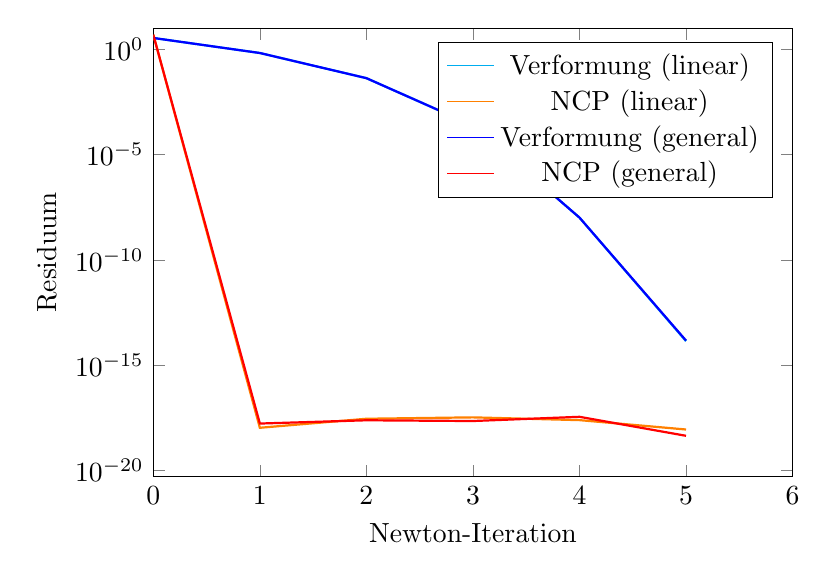
\begin{tikzpicture}[every plot/.append style={thick}] 
\begin{axis}[ 
label style={font=\normalsize}, 
xlabel={Newton-Iteration}, 
ylabel={Residuum}, 
xmin=0, xmax=6, 
ymode=log, 
ymin=0, ymax=10, 
width=0.8\textwidth, 
height=0.6\textwidth, 
legend pos=north east, 
legend style={cells={align=left}}, 
grid style=dashed, 
] 
\addplot[ 
color=cyan, 
] 
coordinates { 
(0, 3.45e+00)(1, 6.66e-01)(2, 4.26e-02)(3, 2.42e-04)(4, 1.02e-08)(5, 1.39e-14)}; 
\addlegendentry{Verformung (linear)} 
\addplot[ 
color=orange, 
] 
coordinates { 
(0, 4.90e+00)(1, 1.07e-18)(2, 2.87e-18)(3, 3.34e-18)(4, 2.47e-18)(5, 8.86e-19)}; 
\addlegendentry{NCP (linear)} 
\addplot[ 
color=blue, 
] 
coordinates { 
(0, 3.45e+00)(1, 6.66e-01)(2, 4.26e-02)(3, 2.42e-04)(4, 1.02e-08)(5, 1.48e-14)}; 
\addlegendentry{Verformung (general)} 
\addplot[ 
color=red, 
] 
coordinates { 
(0, 4.90e+00)(1, 1.70e-18)(2, 2.43e-18)(3, 2.24e-18)(4, 3.55e-18)(5, 4.45e-19)}; 
\addlegendentry{NCP (general)} 
\end{axis} 
\end{tikzpicture} 
\caption{Residuen des Stoffgesetzes 'Neo Hooke' mit Hinderniss 'Spitze' und 578 Freiheitsgraden für die Verschiebung.} 
\label{fiq:NeoHooke_Spitze_level3} 
\end{figure} 
